The  maximum required  output power  of our  device was  roughly calulated  as
$\SI{24}{\volt} \cdot \SI{3}{\ampere} = \SI{72}{\watt}$ (based on the VI-curve
in the specifications,  see appendix \code{TODO}).  Assuming  an efficiency of
$\eta\approx  \SI{90}{\percent}$  an  \SI{80}{W}  power  supply  is  therefore
required.


The design and  construction of a custom power supply  would have consumed too
much time  and resources. The chosen power  supply is mounted inside  the case
and can supply \SI{28}{\volt} at \SI{75}{\watt}.

%\ref{fig:circuit:mains-input}.
%
%\begin{figure}[th!]
%    \centering
%    \begin{minipage}{.3\textwidth}
%        \centering
%        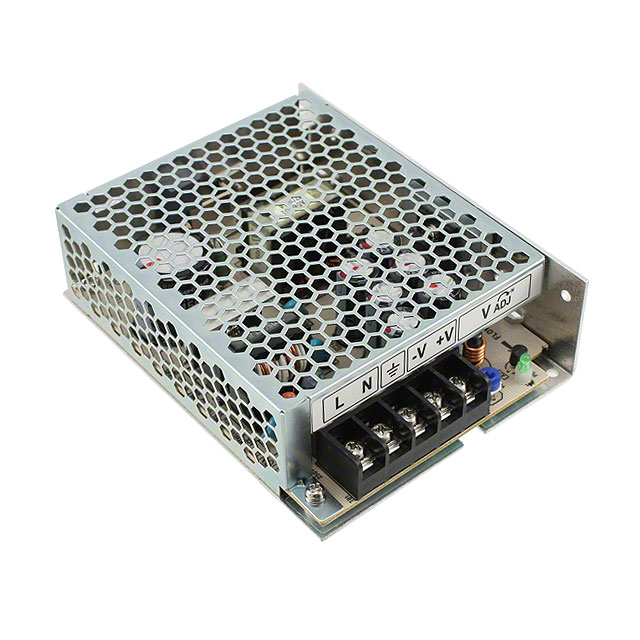
\includegraphics[width=\textwidth]{images/circuit/external-power-supply.JPG}
%        \caption{External PSU}
%        \label{fig:circuit:mains-input}
%    \end{minipage}
%    \begin{minipage}{.3\textwidth}
%        \centering
%        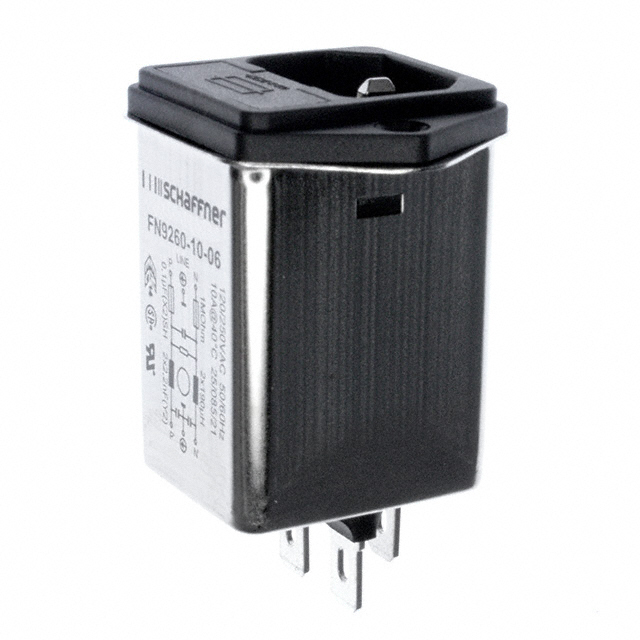
\includegraphics[width=.9\textwidth]{images/circuit/power-entry-module.JPG}
%        \caption{Power Entry Module}
%        \label{fig:circuit:iec60320c13}
%    \end{minipage}
%    \begin{minipage}{.3\textwidth}
%        \centering
%        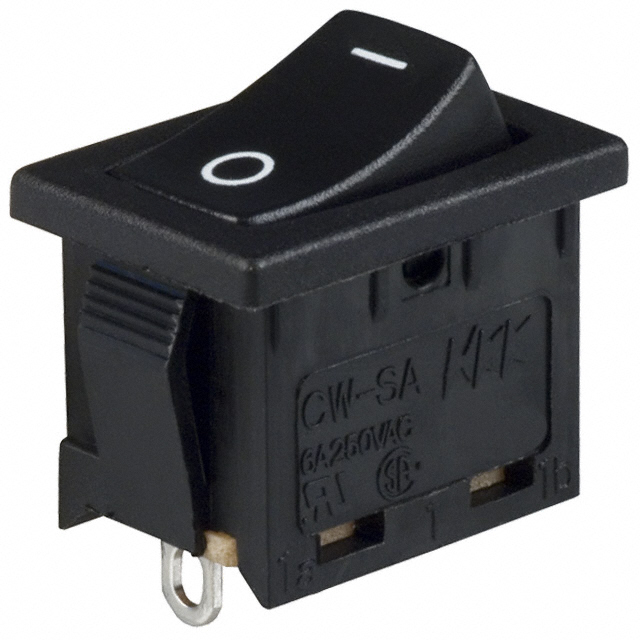
\includegraphics[width=.6\textwidth]{images/circuit/rocker-switch.JPG}
%        \caption{Rocker Switch}
%        \label{fig:circuit:rocker-switch}
%    \end{minipage}
%\end{figure}

It can be plugged  into a power outlet by means of an  IEC 60320 C13 socket
% as seen in figure \ref{fig:circuit:iec60320c13}.
The socket has a built-in fuse as  well as a built-in mains filter, which will
reduce high frequency coupling back into the mains from the device.

A rocker switch
%(figure \ref{fig:circuit:rocker-switch})
is connected in series with the socket  and the power supply, allowing for the
end user to cut power at any time.

\emph{TODO: Show photo of wiring in housing}

